\documentclass{article}

\usepackage{amsmath}
\usepackage{tikz}

\title{CHAPTER 0\\
REVIEW OF ALGEBRA\\ 
01. Sets of Real Numbers
}
\author{Exercised by: Rizal Bimanto}
\date{}

\begin{document}
\maketitle
A set is determined by its elements.
Neither rearrangements neither nor repetitions in a listing affects the set.
A $set A$ is said to be a subset of $set B$ if and only if
every element of $A$ is also an element of $B$.\par

For example, if $A = \left\{ 6, 8, 10 \right\}$ and $B = \left\{ 6, 8, 10, 12 \right\}$,
then $A$ is a subset of $B$. However, $B$ is not a subset of $A$.
There is exactly one set which contains no elements.
It is called the empty set and is denoted by Ø.\par

\section{Real Numbers}
Real numbers are a set of numbers which encompass all the possible
numbers that can be represented on a continous number line.
Real numbers may contain various type of numbers. Such as:
\begin{enumerate}

    \item Rational numbers \par 
    These are the numbers that can be expressed as
    \textbf{ratio of two numbers} (where the denominator is not 0).
    \underline{They can have terminating decimal representations},
    for instances are
    \begin{itemize}
        \item $\frac{3}{4} = 0.75$,
        \item $\frac{1}{5} = 0.4$,
        \item or \underline{non-terminating and repeating decimal numbers}.
        Such as
        \begin{itemize}
            \item $\frac{1}{3} = 0.33333\dots$,
            \item $- \frac{4}{11} = 0.363636\dots$,
            \item and $\frac{2}{15} = 0.13333\dots$
        \end{itemize}
    \end{itemize}

    \item Irrational Numbers \par
    These are the numbers that cannot be expressed as a ratio of two integers.
    The decimal expansion are \textbf{non-terminating} and \textbf{non-repeating}.
    Irrational numbers cannot be written as an integer divided by integer.
    Examples:
    \begin{itemize}
        \item $\pi$ (pi)
        \item $e$ (Euler)
        \item $\sqrt{2}$
        \item $\sqrt{3}$
        \item $\sqrt{5}$
        \item $\varphi$ (Golden Ratio)
    \end{itemize}

    \item Integers: \par
    This is a subset of rational numbers that include zero,
    positive whole numbers (natural numbers), and their negatives. \\
    Examples: \dots, -2, -1, 0, 1, 2, \dots

    \item Whole Numbers: \par
    These include all natural numbers along with zero.

    \item Natural Numbers: \par
    Also known as counting numbers. These starts from 1 and go on indefinitely
    (1, 2, 3, \dots) \par
    
    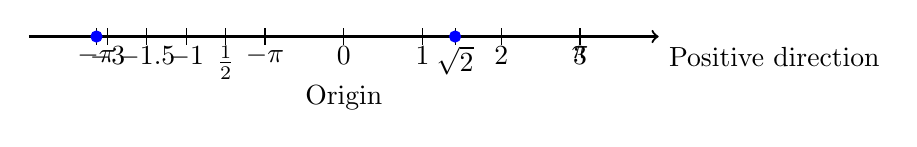
\begin{tikzpicture}
        % Draw the main line
        \draw[thick, ->] (-4,0) -- (4,0) node[anchor=north west] {Positive direction};
    
        % Draw ticks and labels below the line
        \foreach \x/\xtext in {-3.14/-\pi/below, -3/-3/above, -2.5/-1.5/above, -2/-1/above, -1.5/\frac{1}{2}/below, -1/-\pi/below, 0/0, 1/1/above, 1.4142/\sqrt{2}, 2/2, 3/\pi, 3/3}
        {
            \draw[shift={(\x,0)}] (0pt,3pt) -- (0pt,-3pt);
            \node[below] at (\x, 0) {$\xtext$};
        }
    
        % Add origin label
        \node[align=center, below] at (0, -0.5) {Origin};
        
        % Adding bullet points at specified positions
        \foreach \x in {-3.14, 1.4142}
        \filldraw[blue] (\x,0) circle (2pt); % You can change the color and size of the circle
    \end{tikzpicture}
\end{enumerate}
\end{document}